\documentclass[a4paper,11pt,leqno]{report}

\usepackage{amsmath, amssymb, mdframed, caption, subcaption}
\usepackage{nicefrac}
\usepackage{graphicx}
\usepackage{hyperref}
\hypersetup{colorlinks=true, urlcolor=blue, breaklinks=true}

\newmdtheoremenv{Definition}{Definition}[chapter]
\newmdtheoremenv{Exercise}{Exercise}[chapter]
\newmdtheoremenv{Theorem}{Theorem}[chapter]

\title{Basic Probability}
\date{}

\begin{document}

\setcounter{chapter}{2}

\chapter{Random variables and their properties}

\section{What is a random variable?}
\textbf{Random variables} are a tremendously useful concept in probability theory. In most situations of
science and general life we are not really interested in the actual outcome of a random experiment. Instead,
we care about particular properties of that outcome.

For starters, let us talk about the weather. 
Like most people living in the north of Europe, your choice of clothing
probably depends strongly on the weather. Let us assume that you have a thick winter jacket that you
put on when it is cold, a light soft-shell jacket that you wear when temperatures are mild and that you
simply wear a T-shirt or a sweater when it is warm. Let us also assume that the forecasting site you
consult every morning reports the temperatures up to one decimal. The question is: does it matter to you
whether it is $ 5.4 $ or $ 7.3 $ degrees centigrade outside when you make your decision about what to wear?
Most likely you are only interested in whether it is cold, mild or warm. This may obviously vary according
to your own perception of warmth and cold. Here we will assume that it is cold whenever the temperature
is below 10 degrees, mild between 10 and 20 degrees (inclusive) and warm whenever the temperature rises
above 20 degrees. So what you are really interested in, at least as far as clothing is concerned, is 
whether the temperature $ t $ is $ t < 10 $ or $ 10 \leq t \leq 20 $ or $ t > 20 $. What we are looking for
is a way of transforming outcomes from the temperature scale into judgements of perceived temperature.

Another example is the lottery. Let us again consider the Dutch lottery where you have to correctly 
predict 6 out of 49 numbers and one out of 6 colours all which are drawn \textit{independently} 
and \textit{uniformly at random} (you should be able to understand the first term by now; after reading
this chapter, you will also understand the second). You get the main prize if you predict all these items
correctly. However, pay-outs start from three correctly predicted numbers and increase for each additional
number that you got right. So what do you really care about when playing the lottery? Does it matter to
you whether or not you correctly predicted the number 39? Probably not. All you care about is how many of
the numbers you got right.

Observe that one possible way of modelling the sample space for the lottery situation is the following:

\begin{align}
\Omega = \{(b_{1}, \ldots, b_{7}, c_{1}, \ldots, c_{7})| b_{1}, \ldots, b_{6} \in \{1,\ldots, 49\}; \\
i \not = j \Rightarrow b_{i} \not = b_{j};
b_{7} \in \{50, \ldots, 55\}; c_{1}, \ldots, c_{7} \in \{0,1\} \} \nonumber
\end{align}

This rather cumbersome expression states that we draw 6 balls from an urn of 49 balls without replacement,
then draw one ball from an urn of six balls (which we numbered higher than the balls from the first
urn for better discrimination). We also add indicators of whether we predicted each ball drawn correctly.
So again the question arises of how we can transform outcomes from this sample space into
the events that we actually care about (namely how many balls we predicted correctly)?

After this little motivating section, let us now formally define what a random variable is.

\begin{Definition} 
A (real) random variable (RV) is a function
$$ X: (\Omega, \mathcal{A}, \mathbb{P}) \rightarrow \mathbb{R} $$
We additionally require that each set $ A = \{\omega| X(\omega \leq r\} $ be in $ \mathcal{A} $ for
all $ r \in \mathbb{R} $.
\end{Definition}

Notice that the naming of the random variable is arbitrary but by convention we will often use the letters
$ X,Y,Z $. Also, as you can see, RVs operate on an entire probability space. The reason is that
we want to have a probability measure associated with our sample space. 
In fact, this probability measure is the reason why random variables are assuming their values
in a random way. Moreover, since we can only measure events from our events space, the condition on RVs
ensures that we can in fact measure the probability of each real value that we may map an outcome to.
In technical terms, we are thus making sure that the image of the RV is \textit{measurable}.

Let us define a random variable for the weather situation. 
\begin{equation} \label{weatherRV}
X(t) = 
\begin{cases}
1 & t < 10 \\
2 & 10 \leq t \leq 20 \\
3 & t > 2
\end{cases}
\end{equation}

In principle we can now easily determine the probability of each of the values of this RV. However, we did
not bother to define a sample space and associated probability measure, mostly because we would have to
restrict the possible temperatures to those that we think are reasonable. Nevertheless, this is something
that you can do yourself.

\begin{Exercise}
Define an upper and lower bound for temperature values (make sure you can actually get all three perceived
degrees of warmth). This will give you a discrete sample space since we postulated
that the website we consult only reports temperatures up to one decimal place after the comma. Then impose
any probability measure on the associated event space. Finally, compute the probability of each of the
values of the RV $ X $ from eq. \ref{weatherRV}.
\end{Exercise}

We can do the same for the lottery. Our random variable would then look as follows:
\begin{equation}\label{lotteryRV}
X(\omega) = \overset{7}{\underset{i=1}{\sum}} c_{i}
\end{equation}

Whenever a RV assumes a particular value, we write $ X=x $. Thus, if $ X $ in eq. \ref{lotteryRV} assumes the
value $ 4 $, i.e. we guessed for balls correctly, we would write $ X=4 $. And here comes the function
that will officially compute the probability that this happens for us.

\begin{Definition}
The discrete probability distribution of a RV $ X $ is the function
$$ P_{X}(X=x) := \mathbb{P}(\{\omega|X(\omega)=x\}) $$
\end{Definition}

Now what is $ P_{X}(X=4) $ for the lottery example? Recall that there are 
$ a = \binom{49}{6} \times 6 $ sequences of balls that we can draw. Now in the above scenario we also have to take
into account whether or not we correctly predicted each ball, leaving us with a total of $ 2^{a} $
outcomes. At the same time there are $ b = \binom{45}{2} \times 6 + \binom{46}{3} \times 5 $ outcomes in which we have made 
exactly 4 correct predictions. Thus we get $ P_{X}(X=4) = \nicefrac{2^{b}}{2^{a}} $.

We can of course also make statements
like $ X < x $ and $ X \geq x $. This is a way of expressing that a RV assumes a value above or below a certain
threshold. The way to get the probability that this would happen is through the \textbf{cumulative distribution
function}.

\newpage
\begin{Definition}
The cumulative distribution function (cdf) of a random variable $ X $ is given as
$$ F_{X}(a) := P_{X}(X \leq a) = {\underset{x \leq a}{\sum}}P(X=x) $$
\end{Definition}

The cumulative distribution function is helpful in two ways. First of all, it allows us to get the probability that
$ X $ takes on a value in a certain range. Second, it has applications in sampling algorithms, some of which we might
see during the programming part of the course. A plot of the cdf of $ Z $ is given in Figure~\ref{cdfPlot}. We can recognize that it is the cdf of a discrete
distribution because it is discontinuous. If the underlying probability distribution was continuous, so would be its cdf.

\begin{figure}
\center
<<<<<<< Updated upstream
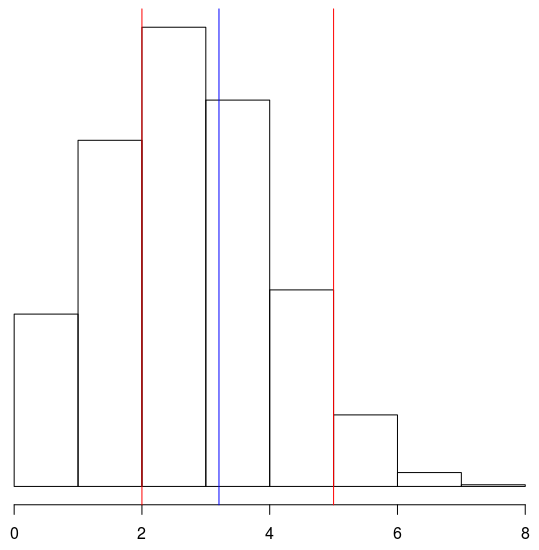
\includegraphics[scale=.3]{histogram.png}
\caption{Probability distribution of a random variable with $ 8 $ possible values.}
=======
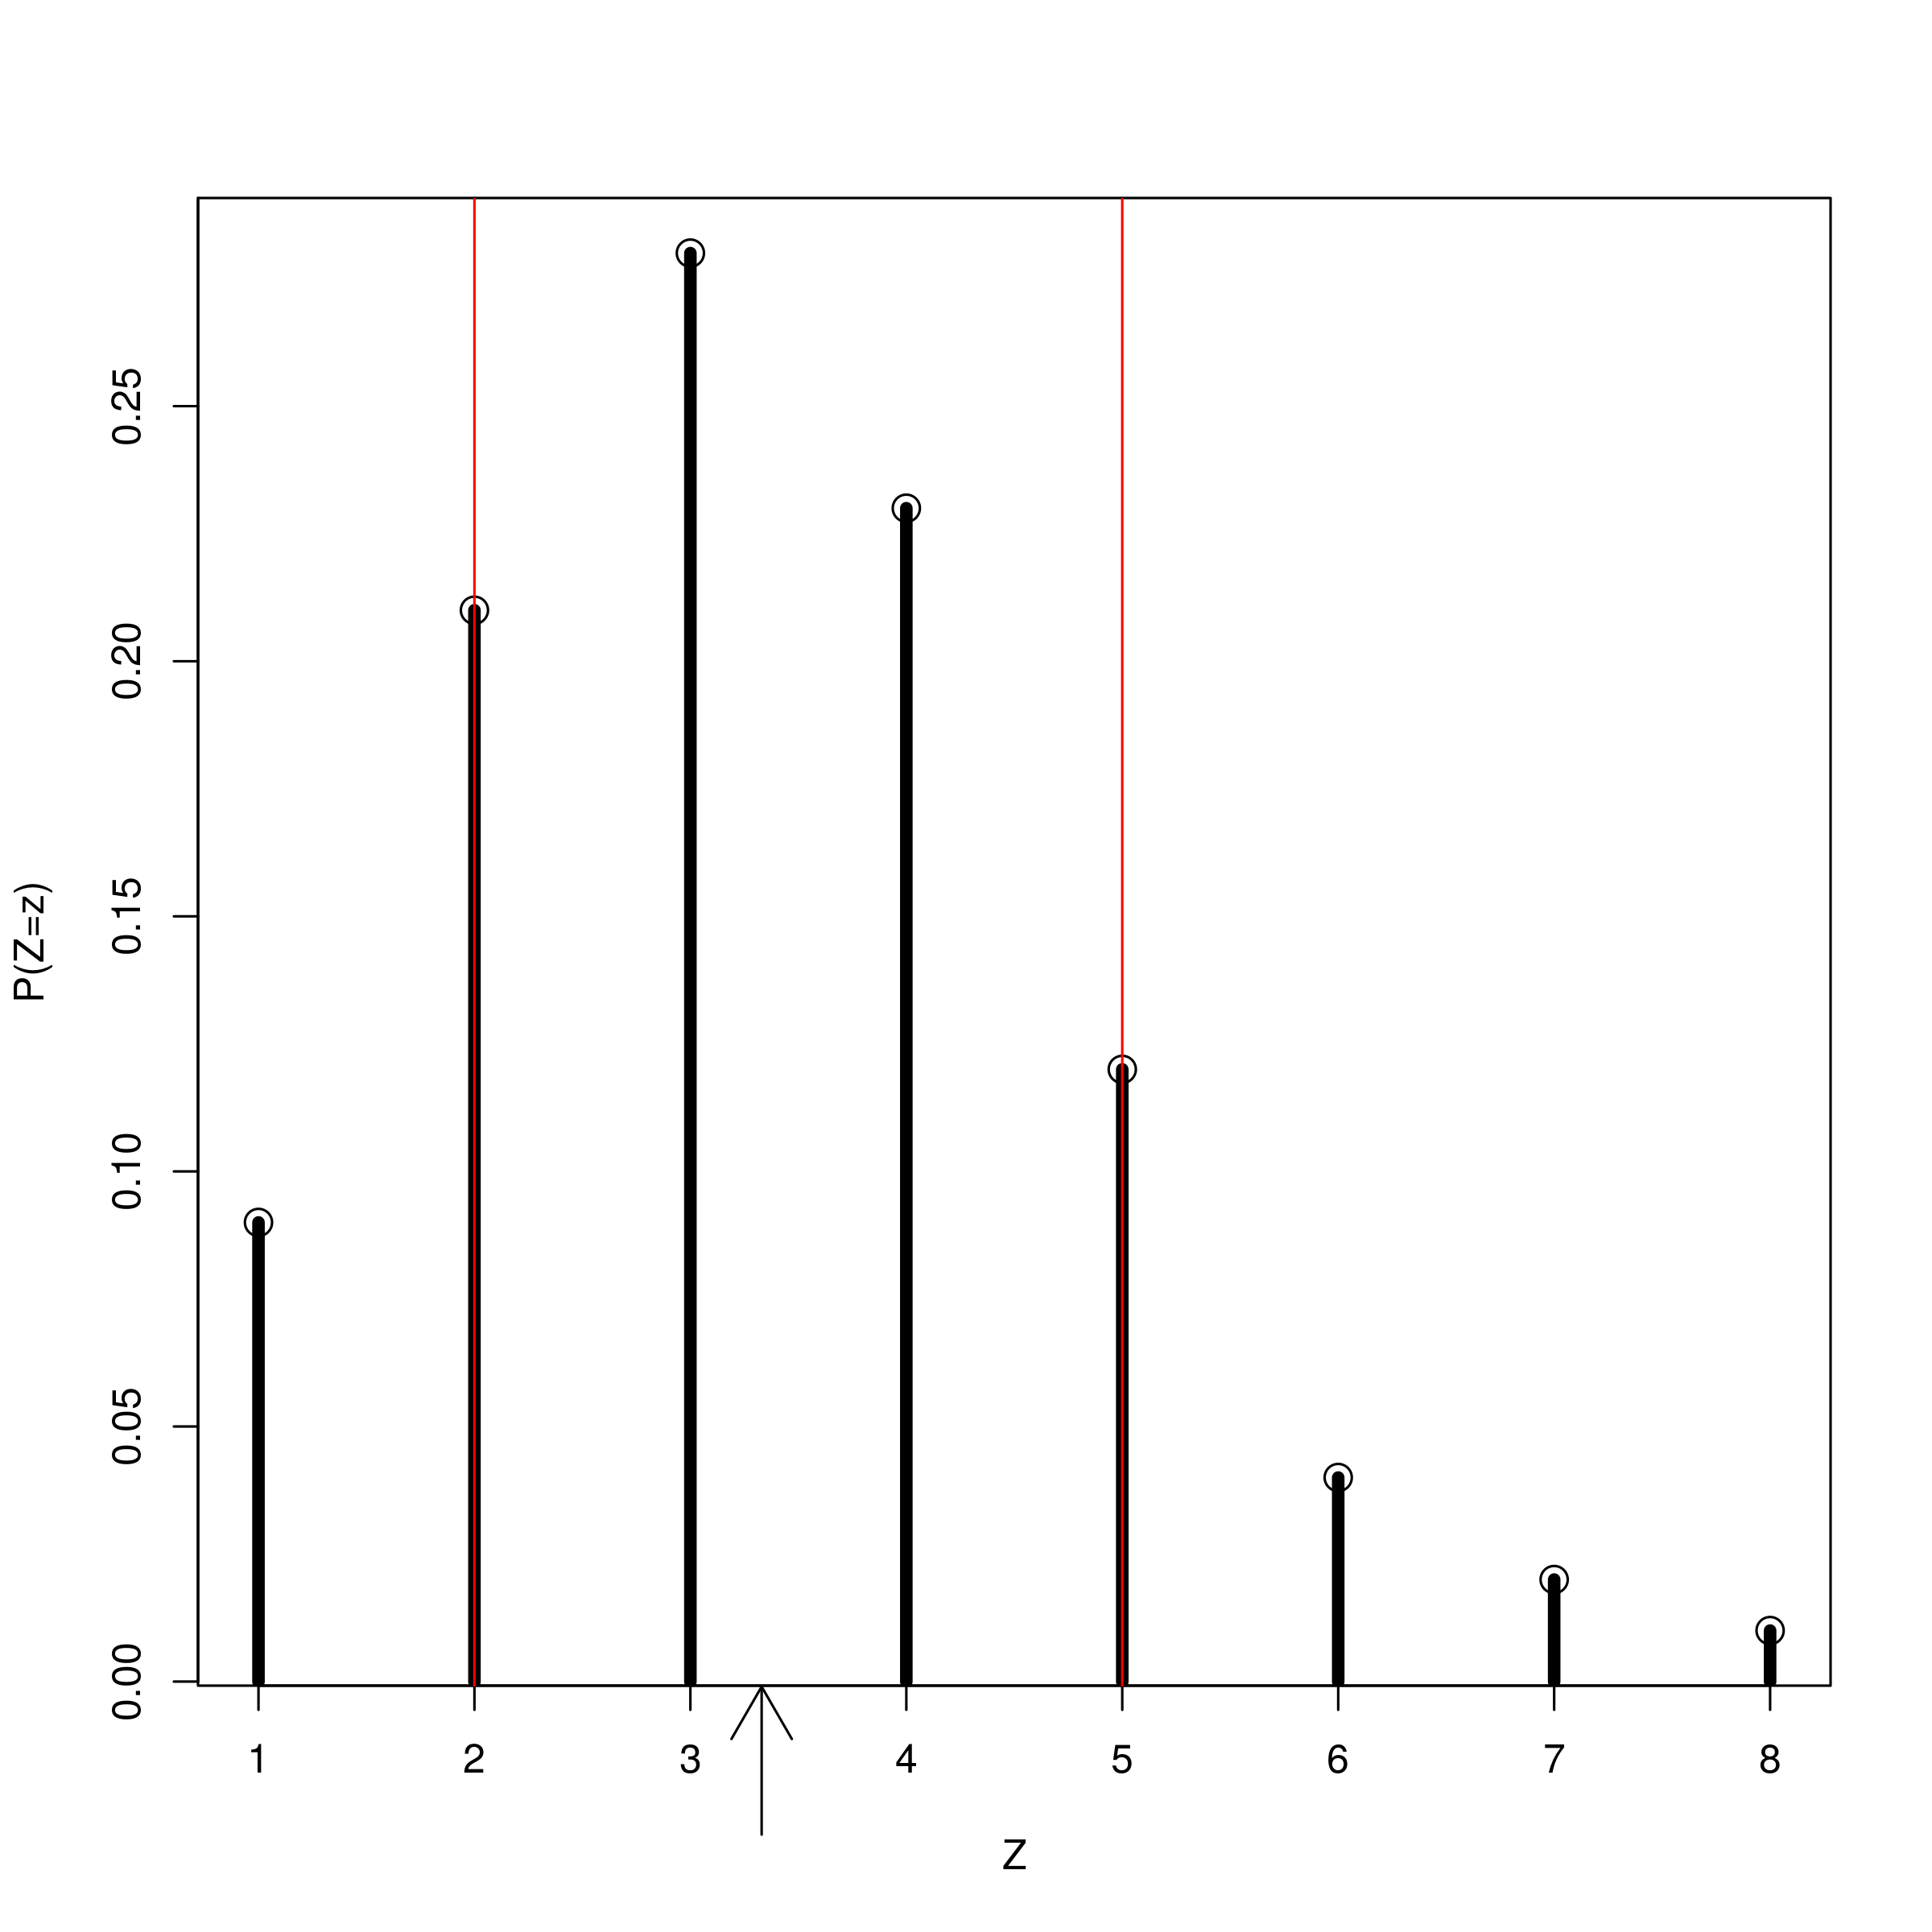
\includegraphics[scale=.4]{distribution.png}
\caption{\chris{It should rather be a bar plot instead of a histogram, like~\url{http://www.math.uah.edu/stat/expect/DiscreteCenterMass.png}, because the mass is concentrated in discrete points.} Probability distribution of a random variable $Z$ with $ 8 $ possible values, given by $ P(Z = 1) = 0.09,  P(Z = 2) = 0.21, P(Z = 3) = 0.28, P(Z = 4) = 0.23, P(Z = 5) = 0.12, P(Z = 6) = 0.04, P(Z = 7) = 0.02$, and $ P(Z = 8) = 0.01$. The arrow indicates the expectation. This is a visualisation of 
the spike that we can plug underneath the centre of mass.}
>>>>>>> Stashed changes
\label{binomplot}
\end{figure}

\begin{figure}
\center
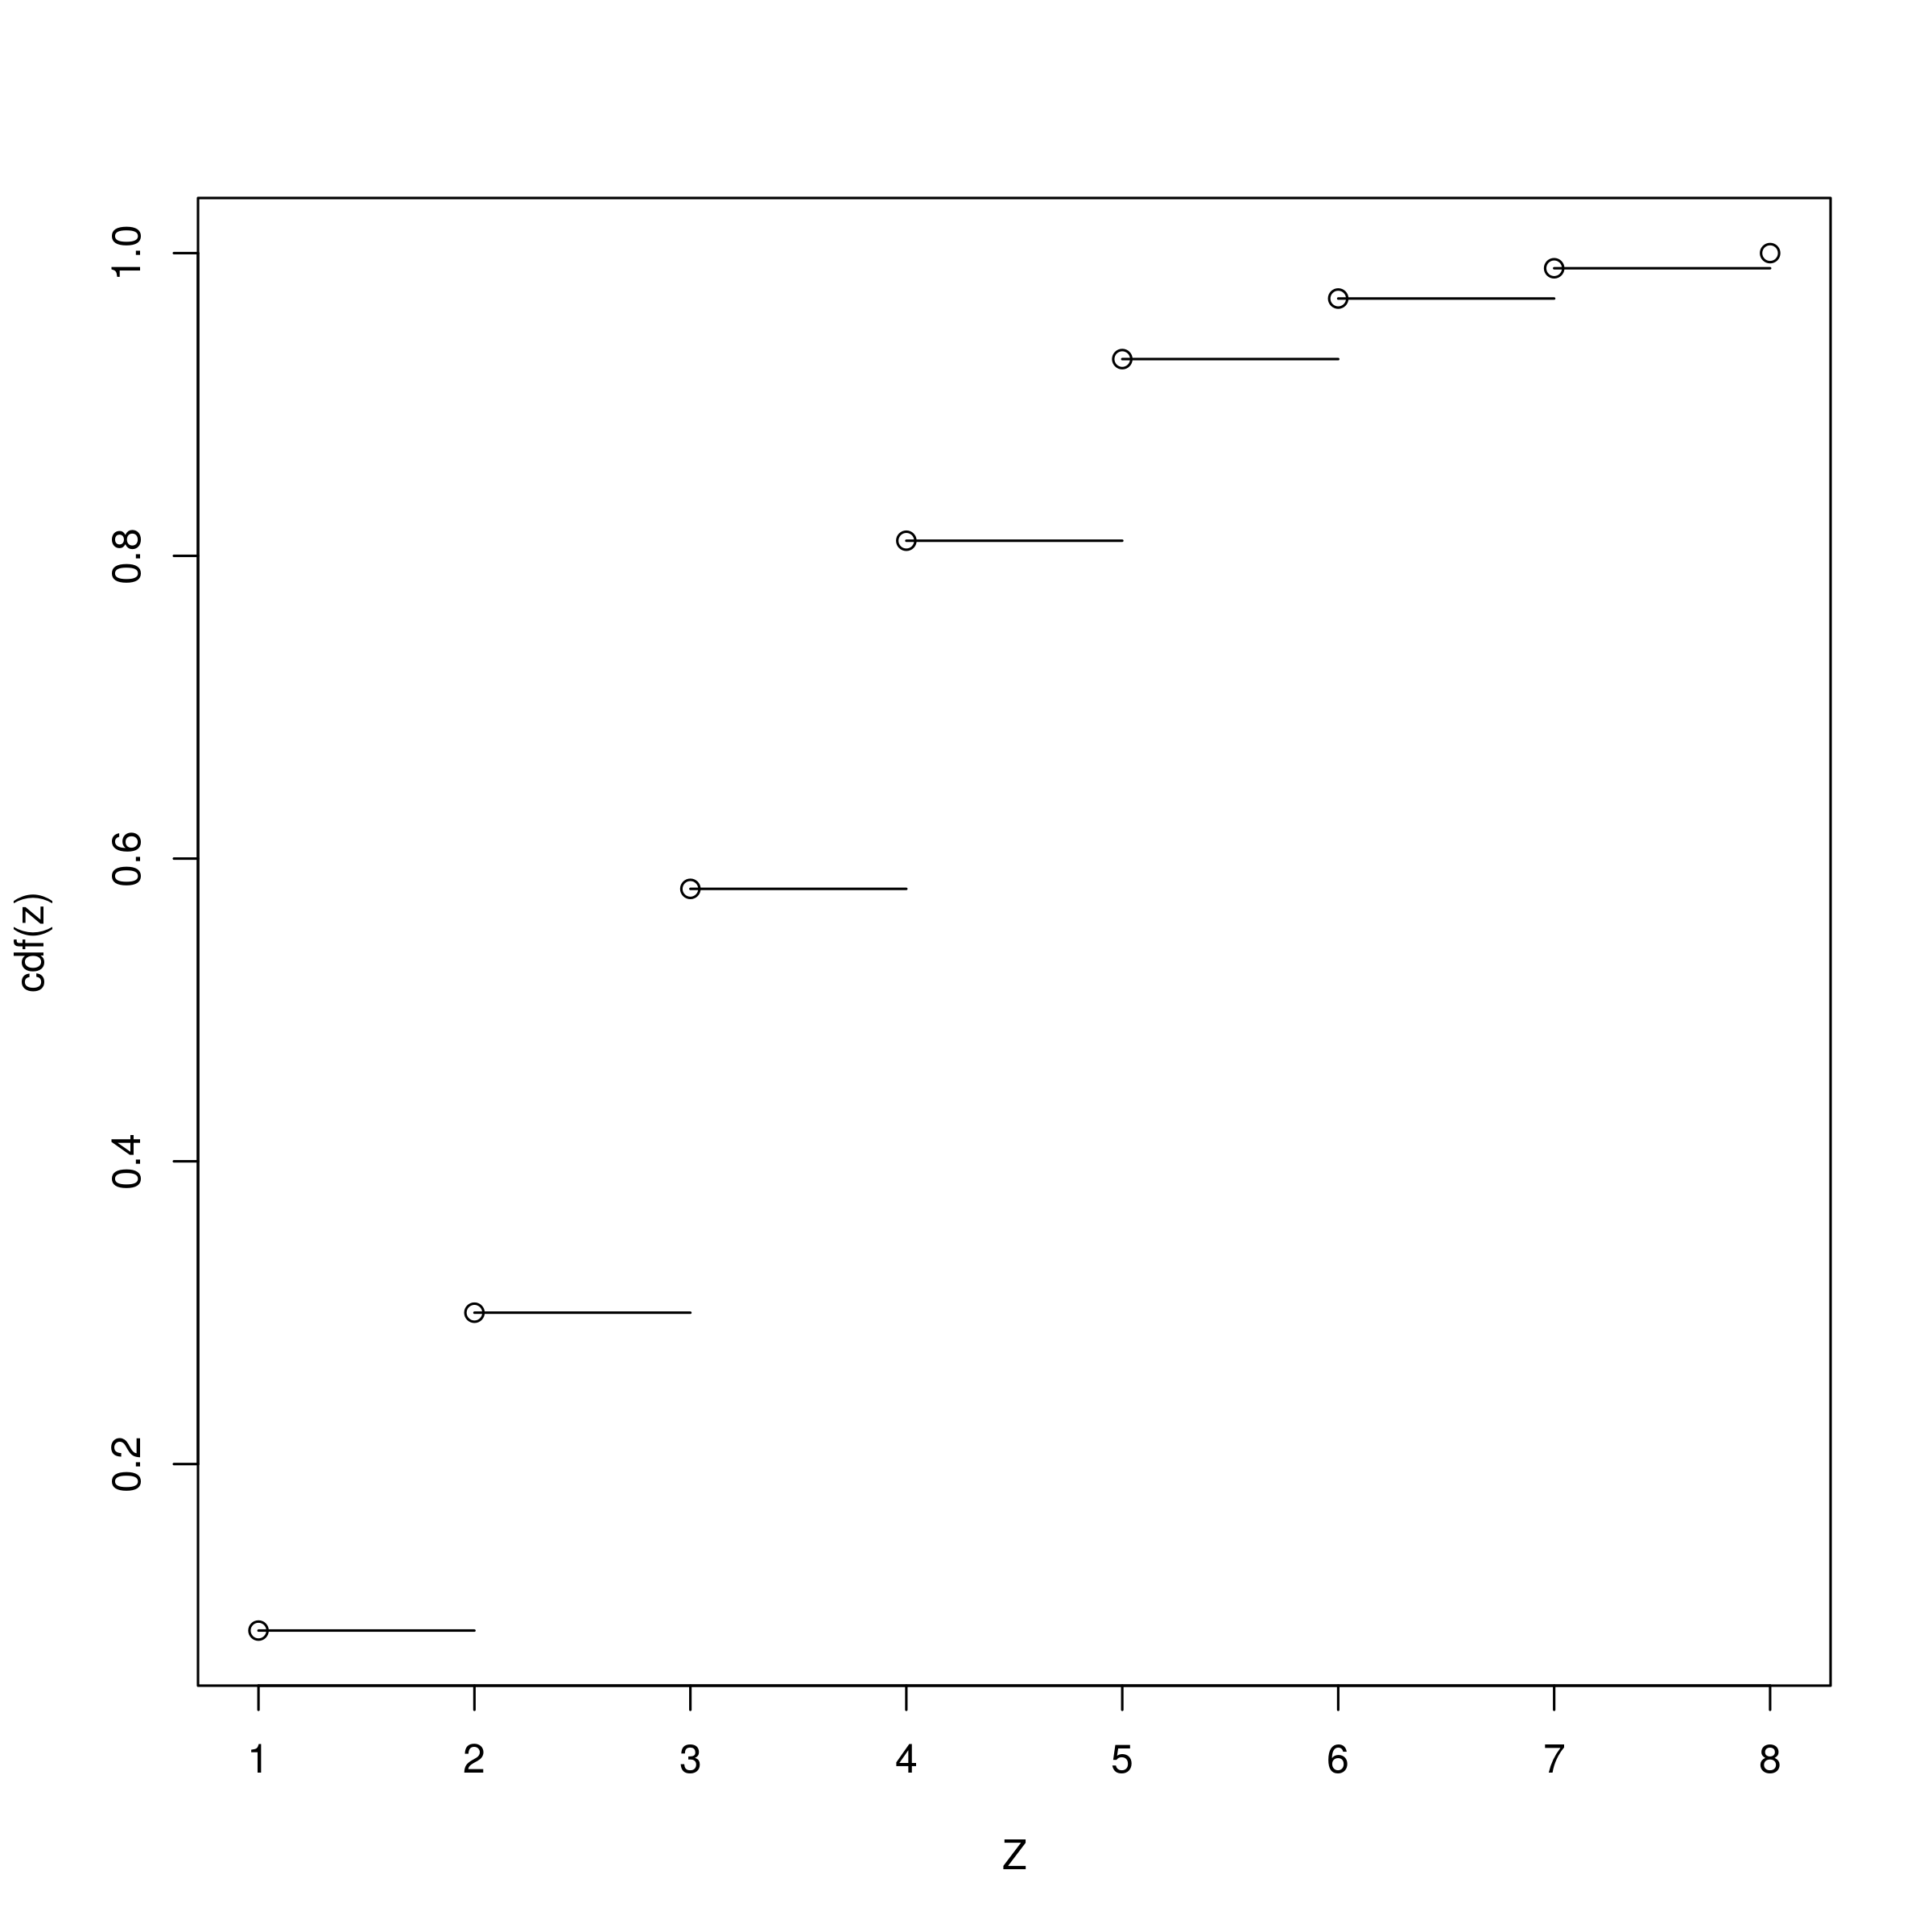
\includegraphics[scale=.4]{cdf.png}
\caption{Cumulative probability distribution of $ Z $. Observe that it stays constant in values that $ Z $ cannot take on. This cdf being discontinuous is an indicator
that the underlying probability distribution is discrete.}
\label{cdfPlot}
\end{figure}

To better understand how we can compute the probability that $ a \leq X \leq b $ for some real values $ a,b $ let us take a 
look at fig. \ref{binomplot}. There we see a plot of the probability distribution of a random variable $ Z $. The red lines
indicate the interval that we are interested in. As a warm-up exercise, let us first compute $ P_{Z}(Z \leq 2) $ and 
$ P_{Z}(Z > 5) $. By looking at the plot we easily see which areas we need to consider, namely the bars to the left of 2
and to the right of 5. The height of the bars corresponds to their probability. The probability distribution is given as
\begin{itemize}
\item $ P_{Z}(Z = 1) = 0.09 $
\item $ P_{Z}(Z = 2) = 0.21 $
\item $ P_{Z}(Z = 3) = 0.28 $
\item $ P_{Z}(Z = 4) = 0.23 $
\item $ P_{Z}(Z = 5) = 0.12 $
\item $ P_{Z}(Z = 6) = 0.04 $
\item $ P_{Z}(Z = 7) = 0.02 $
\item $ P_{Z}(Z = 8) = 0.01 $
\end{itemize}

We go on to compute the probability that $ Z $ is smaller or equal to 2 and that $ Z $ is bigger or equal to 5.

\begin{align}
P_{Z}(Z \leq 2) =& P_{Z}(Z=1) + P_{Z}(Z=2) = 0.09 + 0.21 = 0.3 \\
P_{Z}(Z > 5) =& P_{Z}(Z=6) + P_{Z}(Z=7) + P_{Z}(Z=8) \\ 
=& 0.04 + 0.02 + 0.01 = 0.07 \nonumber
\end{align} 

Now it is straightforward to compute $ P_{Z}(2 < Z \leq 5) $. If we again look at fig. \ref{binomplot} we see that this is
the area delimited by the red lines. Thus, $ P_{Z}(Z \leq 5) $ will be an overestimate of this probability. The amount by
which it is an overestimate is exactly $ P_{Z}(Z \leq 2) $. Thus we get $ P_{Z}(2 < Z \leq 5) = P_{Z}(Z \leq 5) - P_{Z}(Z \leq 2) $.

\begin{Exercise}
We claim that you can compute $ P_{Z}(2 < Z \leq 5) $ based on $ P_{Z}(Z \leq 2) $ and $ P_{Z}(Z > 5) $ from above. What result do
you get?
\end{Exercise}

In the case of discrete random variables, i.e. the ones that we are dealing with here, there is another function that is of great 
interest, namely the \textbf{probability mass function}.

\begin{Definition}
The probability mass function (pmf) of a random variable $ X $ is given as
$$ p(x) := P_{X}(X = x) $$
\end{Definition}

The pmf is notationally more convenient than the probability distribution but also less general. For example, the pmf does not
allow us to express that $ X $ falls in a range of values. In order to avoid confusion, we will mostly use $ X $'s 
probability distribution here. Be aware, however, that most papers that you are going to read in the future will use the pmf
instead. Regardless of whether we are using the probability distribution or the pmf, we will call the values in $ \mathbb{R} $
to which they assign positive probability, their \textbf{support}.



\section{Expectation and Variance}

There are two major properties of probability distributions that are used to describe them. One is the center of mass, the point
at which the probability mass of the distribution is split into half. If you think of the support of $ P_{X} $ as a plank and 
of the probabilities as weights, then the center of mass is the point at which you could put an infinitely thin spike into the
plank from underneath such that the plank maintains perfect balance. In fig. \ref{binomplot} this so-called \textbf{expectation}
is indicated by the blue line.

<<<<<<< Updated upstream
\begin{Definition}
The expectation of a random variable $ X $ with respect to the distribution $ P_{X} $ is defined as
$$ E_{P_{X}}[X] := \underset{i = 1}{\overset{|X|}{\sum}} x_{i}P_{X}(x_{i}) $$
where $ |X| $ is the size of the support of $ X $ and $ x_{i} $ are the members of that support.
=======
\begin{Definition}[Expectation]
The \textbf{expectation} of a random variable $ X $ with respect to the distribution $ P $ is defined as
$$ \E[X] := \sum_{x \in \supp(X)} x P(X=x) $$ \, . \philip{Are you sure you want to have this dot here? It seems to unnecessarily inflate the box.}
>>>>>>> Stashed changes
\end{Definition}

\begin{Exercise}
Compute the expectation of the random variable $ Z $ from the previous section.
\end{Exercise}

It is important to point to the fact that the expectation is a theoretical quantity. This implies that
it does not need to be a value in the support of $ X $. This is for example the case in fig. \ref{binomplot} where the
expectation is fractional although all support values are integers.

The expectation comes with an interesting property that is called the \textbf{linearity of expectation}. Basically whenever
we multiply $ X $ with a constant $ a $ the expectation will be scaled by that constant. Moreover, when we add a constant $ b $
to $ X $ the expectation will also increase/decrease by $ b $ (depending on whether $ b $ is positive or negative). Let's
proof that!

\begin{align}
E_{P_{X}}[aX+b] &= \underset{i = 1}{\overset{|X|}{\sum}} a(X=x_{i}+b) P_{X}(x_{i}) \\
&= a \underset{i = 1}{\overset{|X|}{\sum}} (x_{i}+b) P_{X}(X= x_{i}) \\
&= a \underset{i = 1}{\overset{|X|}{\sum}} x_{i}P_{X}(X=x_{i})+bP_{X}(X=x_{i}) \\
&= a \underset{i = 1}{\overset{|X|}{\sum}} x_{i}P_{X}(X=x_{i}) + \underset{i = 1}{\overset{|X|}{\sum}}bP_{X}(X=x_{i}) \\
&= a \underset{i = 1}{\overset{|X|}{\sum}} x_{i}P_{X}(X=x_{i}) + b \label{sumToOne} \\
&= a E_{P_{X}}[X]+b 
\end{align}

The equality in \ref{sumToOne} follows from the fact that the sum of the probabilities of the support of a distribution is 1.
The linearity of expectation is extremely useful. Basically, if you know the expectation of a RV you also know the 
expectation of its multiples. Furthermore, by adding a constant, we basically shift each element in the support. However, this shifting
does not do anything surprising as the centre of mass shifts by the same amount.

We can actually take the expectation of any quantity. However, this only makes sense for quantities that
can be cast as functions of $ X $. The expectation of a quantity that is constant with respect to $ X $ will just be that
quantity itself. More formally:
\begin{equation}
E_{P_{X}}[a] = \underset{i = 1}{\overset{|X|}{\sum}} aP_{X}(X=x_{i}) = a
\end{equation}

A class of functions of $ X $ that people are often interested in are the moments. Moments are the powers of $ X $, so $ X $ itself
is the first moment $ X^{2} $ is the second moment and so on. We will not further discuss moments here but it is useful to at
least know what they are in case you find the expression in a paper.

After we have discussed the centre of mass, it is also interesting to look at how far away the average outcome (or rather its image
under the random variable) is from it. Assume two random variables $ X $ and $ Y $ with
\begin{itemize}
\item $ P_{X}(X=-100) = 0.5 $; $ P_{X}(X=100) = 0.5 $
\item $ P_{Y}(Y=-1000) = 0.5 $; $ P_{Y}(Y=1000) = 0.5 $
\end{itemize}
The spread of $ Y $ is obviously going to be greater, although both have the same expectation. The quantity usually used to assess
the spread of a RV is the \textbf{variance}.

\begin{Definition}
The variance of a RV $ X $ with distribution $ P_{X} $ is given as
$$ var(X) := E_{P_{X}}[(E_{P_{X}}[X] - X)^{2}] $$
\end{Definition}

The expression for $ var(X) $ is rather scary-looking but let us try to make sense of it. The inner part is the difference between
each value of the random variable and the expectation. Thus the out expectation is just a weighted sum of differences between 
values in the support and the expectation. However, since values of $ X $ can be smaller or greater than the expectation, this
sum will be 0. Therefore we square it, leaving us only with positive values. In sum, the variance is the expectation
of the squared differences between the expectation and the values in the support of $ X $.

Computing the variance as an expectation can be cumbersome. We will now show how it can be done more efficiently.
\begin{align}
var(X) &= E_{P_{X}}[(E_{P_{X}}[X] - X)^{2}] \\
&= \underset{i = 1}{\overset{|X|}{\sum}} P_{X}(X=x_{i}) (E_{P_{X}}[X] - X)^{2} \\
&= \underset{i = 1}{\overset{|X|}{\sum}} P_{X}(X=x_{i}) (E_{P_{X}}[X])^{2} - 2XE_{P_{X}}[X] + X^{2}) \\
&= (E_{P_{X}}[X])^{2} - \underset{i = 1}{\overset{|X|}{\sum}} P_{X}(X=x_{i}) 2XE_{P_{X}}[X]
+  \underset{i = 1}{\overset{|X|}{\sum}} P_{X}(X=x_{i})  X^{2} \\
&= (E_{P_{X}}[X])^{2} -  2(E_{P_{X}}[X])^{2} +  E_{P_{X}}[X^{2}] \\
&= E_{P_{X}}[X^{2}] - (E_{P_{X}}[X])^{2} \label{variance}
\end{align}

For most intents and purposes we will use \ref{variance} to compute the variance. Also, from here on, we will generally drop the 
subscript indicating the distribution of the the expectation in order to save ourselves some writing.

\begin{Exercise}
<<<<<<< Updated upstream
Compute the variance of the lottery RV from the previous section.
=======
Compute the variance of the RV Z from the previous section.
>>>>>>> Stashed changes
\end{Exercise}

Although variance is not linear, we can still try to figure out what happens when we multiply a RV by a constant or add a constant to it.
\begin{align}
var(aX+b) &= E[(aX+b)^{2}] - (E[aX+b])^{2} \\
&= E[(aX+b)^{2}] - (aE[X]+b)^{2} \\
&= E[a^{2}X^{2} + 2abX + b^{2}] - a^{2}E[X]^{2} - 2abE[X] - b^{2} \\
&= a^{2}E[X^{2}] + 2abE[X] + b^{2} - a^{2}E[X]^{2} - 2abE[X] - b^{2} \\
&= a^{2}E[X^{2}] - a^{2}E[X]^{2} = a^{2}var(X) \
\end{align}

What we see here is that the variance is not affected by constant additions to the RV. This makes sense, as constant additions just shift
the expectation. However, the relation of each individual value to the expectation is not affected by that. On the other hand,
when we multiply each value of the RV by a constant, the variance is scaled by the square of that constant. Again, this is not surprising.
Remember that we used squaring in our definition of the variance to turn all distances from the expectation into positive numbers.
Now if we multiply an RV by a constant $ a $ its spread will increase in both directions by a factor of $ a $. 
And since we again want only positive differences,
we better square that increased spread. This intuitively justifies the above equalities.



\section{Joint and conditional distributions}

Up to now, we have only looked at cases that could be treated with one random variable. Most interesting problems involve a multitude
of RVs, however. We therefore introduce the concept of \textbf{jointly distributed random variables}. What this means is that
there is a distribution over tuples of values, each from a different RV.

\begin{Definition}
Random variables $ X_{1}, \ldots, X_{n} $ (abbreviated as $ X^{n}_{1} $) 
are said to be jointly distributed with probability distribution $ P_{X_{1}^{n}} $ such that
$$ P_{X^{n}_{1}}(X_{1}=x_{1}, \ldots, X_{n}=x_{n}) = \mathbb{P}(\{\omega|X_{1}(\omega) = x_{1}, \ldots, X_{n}(\omega)=x_{n}\}) $$
\end{Definition}

From the above definition we see that the random variables need to share an underlying sample space. This also gives us more
insight into the real power of RVs: in applications we usually do not care at all about the underlying sample space but only about
certain quantities captured by the RVs. In fact, we may not even be sure what the underlying sample space is and how we would
draw samples from it. Therefore, we simply define a probability distribution over the random variables of interest. Since by definition
the distribution is linked to a probability space, we can rest assured that we are working with a suitable sample space without
having to bother what that space looks like.

Joint distributions are of particular interest because they make it possible to recover the probability distribution of each individual
RV as well as of smaller joint distributions. The process by which this can be accomplished is known as \textbf{marginalization}. Say
we are given a joint distribution $ P_{XY} $. Now how can we determine the probability that $ X=x $? Our sample space is carved
up by the values that $ X $ and $ Y $ can take on. We are interested in the probability of the subset $ E = \{\omega|X(\omega)=x\} $.
Assuming that $ Y $ can take on $ n $ values, let us define $ E_{i} = \{\omega| Y(\omega) = y_{i}\} $ for $ 1 \leq i \leq n $.
Some (possibly all) of the $ E_{i} $ will overlap with $ E $. Thus we can partition $ E $ into $ E\cap E_{1}, \ldots, E \cap E_{n} $.
Now by countable additivity we simply need to sum up the probabilities of these intersections. Observe that those probabilities
correspond exactly to $ P_{XY}(X=x,Y=y_{1}), \ldots, P_{XY}(X=x,Y=y_{1}) $. Hence, we get to the following equality:

\begin{equation} \label{simpleMarginal}
P_{X}(X=x) = \overset{n}{\underset{i=1}{\sum}} P_{XY}(X=x,Y=y_{i}) 
\end{equation}

Now if we set $ X = (Z_{1}, \ldots, Z_{m}) $, we can recover $ P_{Z_{1}^{m}} $ from $ P_{YZ_{1}^{m}} $ in the same way. Likewise,
if we set $ Y = (Z_{1}, \ldots, Z_{m}) $ we get the generalization of \ref{simpleMarginal}. We will assume that each $ Z_{j} $
can assume $ n_{j} $ values.

\begin{align}
P_{X}(X=x) = \overset{n_{1}}{\underset{j_{1}=1}{\sum}}\ldots \overset{n_{m}}{\underset{j_{m}=1}{\sum}} 
P_{XZ_{1}^{m}}(X=x,Z_{1}=z_{j_{1}}, \ldots, Z_{m}=z_{j_{m}})
\end{align}

For exercise purposes, it often helps to draw a joint probability table and do marginalization from there.

\begin{table}
\center
\begin{tabular}{|c|c|c|c|}
\hline
$X\backslash Y$	& 1		& 2		& 3		\\
\hline
1				& 0.15	& 0.08	& 0.07	\\
2				& 0.01	& 0.2	& 0.03	\\	
3				& 0.28	& 0.17	& 0.09	\\
\hline
\end{tabular}
\caption{Joint probability table for $ X $ and $ Y $.}
\label{jointTable}
\end{table}

\begin{Exercise}
Find the marginal distributions $ P_{X} $ and $ P_{Y} $ in table \ref{jointTable}.
\end{Exercise}

We have already seen how the joint probability of random variables links back the the probability space that underlies them.
This makes it easy for us to import certain concepts that we have gotten to know in previous chapters. In particular, we can
define \textbf{conditional probability distributions}.

\begin{Definition}
The probability of $ X = x $ conditioned on $ Y=y $ is given as
$$ P_{X|Y}(X=x|Y=y) = \dfrac{P_{XY}(X=x, Y=y)}{P_{Y}(Y=y)} $$
\end{Definition} 

\begin{Exercise}
Compute the conditional probability distributions $ P_{X|Y=2} $ and $ P_{Y|X=1} $ from table \ref{jointTable}.
\end{Exercise}

Likewise, we can carry over the concept of independence.

\begin{Definition}
Two random variables $ X,Y $ are independent (write: $ X \bot Y $) if $ P_{XY}(X=x, Y=y) = P_{X}(X=x)P_{Y}(Y=y) $.
\end{Definition}

As with events, independence also implies that $ P_{X|Y} = P_{X} $. Moreover, independence makes it much easier for us
to calculate the expectation and variance of jointly distributed random variables. We have to be careful, though. We
cannot just compute the expectation of the joint random variables themselves as it is unclear what this would even be.
What we can do is to compute the expectation of functions of them. The standard choice in the case of expectation
is to simply multiply the RVs.
\begin{align}
E[XY] &= \underset{i=1}{\overset{n}{\sum}}\underset{j=1}{\overset{m}{\sum}} P_{XY}(X=x_{i},Y=y_{j}) x_{i}y_{j} \\
&= \underset{i=1}{\overset{n}{\sum}}\underset{j=1}{\overset{m}{\sum}} P_{X}(X=x_{i})P_{Y}(Y=y_{j}) x_{i}y_{j} \\
&= \underset{i=1}{\overset{n}{\sum}}P_{X}(X=x_{i})x_{i} \underset{j=1}{\overset{m}{\sum}} P_{Y}(Y=y_{j}) y_{j} \\
&= E[X]E[Y]
\end{align}

Similarly it does not really make sense to talk about the variance of two random variables (at least not as one single
value). However, we can again compute the variance of functions. For addition, independence again makes our lives
much easier.

\begin{Exercise}
Show that $ var(X + Y) = var(X) + var(Y) $.
\end{Exercise}



<<<<<<< Updated upstream
\section{Two important distributions}
=======
\section{Three Important Distributions}
>>>>>>> Stashed changes

We will finish this chapter by introducing two extremely useful discrete distributions. They are very often used in
computer science to model the probability of bit strings and linguistics and natural language processing to model
the probability of sentences. 

To get us started let us consider coin tosses. When you toss a fair coin the probability that it lands on heads is 0.5 and
so is the probability that it lands on tails. Let $ 1 $ stand for heads and $ 0 $ for tails in a random variable $ X $ 
modelling coin tosses. Then we can formalize this distribution as
\begin{equation}
P_{X}(X=x) = 0.5^{x}\times 0.5^{1-x}
\end{equation}

Notice though that not all coins are fair and that in general we want to allow for probabilities that are not equal. 
We will therefore introduce a parameter $ \theta $ that regulates the probability that we would observe heads. In the
above equation we set $ \theta = 0.5 $. What happens if we set $ \theta = 0.3 $?
\begin{equation}
P_{X}(X=x) = 0.3^{x} \times 0.7^{1-x}
\end{equation}

Where did we get the 0.7 from? Well, we know that the coin has to land on either heads or tails. Thus, if the probability
to land on heads is $ 0.3 $ the probability to land on tails has to be $ 0.7 $. Moreover, we chose $ 1 $ as a stand-in for
landing on heads. As we would expect, $ X = 1 $ will return the $ 0.3 $ probability and $ X = 0 $ will return the probability of $ 0.7 $.

This leads to a general formulation where we do not specify the parameter $ \theta $ but leave it to be filled in. 
The resulting distribution, known as \textbf{Bernoulli distribution} (with parameter $ \theta $), is shown in eq. \ref{Bernoulli}.
\begin{equation}\label{Bernoulli}
P_{X}(X=x) = \theta^{x} \times (1 - \theta)^{1-x}
\end{equation}

The Bernoulli is defined for one coin flip, or more generally for the drawing of a coloured ball from an urn containing balls
of exactly two colours. Now what if we draw balls repeatedly with replacement? We will get a sequence of coloured balls. 
Say we draw $ n $ balls and repeat this procedure five times. Chances are that the five sequences will look rather different.
<<<<<<< Updated upstream
Thus, we can define a probability distribution over sequences of coloured balls of length $ n $. This can be achieved in a simple generalization
of the Bernoulli. Whereas in the Bernoulli we made one draw we now make $ n $ draws.
\begin{equation}\label{Multinoulli}
P_{X}(X=x) = \theta^{x} \times (1 - \theta)^{n-x}
=======
Thus, we can define a probability distribution over sequences of
coloured balls of length $ n $. This procedure can be described as a simple generalization
of the Bernoulli. Whereas in the Bernoulli we made one draw we make $
n $ draws. This yields a sequence $ x $ in which each position $ x_{i}, 1 \leq i \leq n $ is either $ 0 $ or $ 1 $.
\begin{equation}\label{Multinoulli}
P(X=x) = \theta^{\sum_i x_i} \times (1 - \theta)^{n-\sum_i x_i}
>>>>>>> Stashed changes
\end{equation}

The adjustment is slight. We basically only introduce an extra parameter, namely the number of draws $ n $. 
However, there are two conditions for this distribution that we have not mentioned yet. First and foremost,
the repeated Bernoulli draws are assumed to be independent. That is, for each draw in the sequence it should not matter which colours you
have drawn so far and which ones you are still going to draw. More formally, if we encode each draw in the sequence as a random
variable we postulate that these random variables are independent of each other. 

<<<<<<< Updated upstream
The second point is that we cannot assign a probability to any sequence that contains more ball of one colour than there are balls in total.
This is to say that we require that $ 0 \leq x \leq n $ which is a reasonable restriction. 

It is also worth mentioning that in general the two values that the distributions in \ref{Bernoulli} and \ref{Multinoulli} range
over are generally referred to as success and failure where the success is usually encoded as $ 1 $ and the failure as $ 0 $
(although nothing hinges on that). 
=======
The second point is that we cannot assign a probability to any sequence that contains more balls of one colour than there are balls in total.
This is to say that we require that $ 0 \leq \underset{i=1}{\overset{n}{\sum}}x_{i} \leq n $ which is a reasonable restriction. 

It is also worth mentioning that in general the two values that the distributions in \eqref{Bernoulli} and \eqref{Multinoulli} range
over are generally referred to as success and failure where the success is usually encoded as $ 1 $ and the failure as $ 0 $. 
>>>>>>> Stashed changes

\begin{Exercise}
Use the distribution in eq. \ref{Multinoulli} with $ n = 10 $ and $ \theta = 0.8 $ to determine the probability of the sequence (0,0,1,1,0,1,1,1,0,1).
\end{Exercise}

Another interesting observation is that, since the value at each position in the sequence is independent of all others, all sequences with the same
number of successes and failures will have the same probability. At this point it is natural to ask for the probability to get \textit{any}
sequence with that amount of successes and failures. Say we are dealing with sequences of length $ n $ and wonder about the probability of 
obtaining a sequence with $ 0 \leq x \leq n $ successes. Then we simply need to count up the probabilities of all sequences that contain $ x $ 
successes. But how many such sequences are there? If you recall chapter 1, there we talked about how to choose a subset of $ k $ elements
out of $ n $. This is exactly the problem we are facing here. We want to know how many ways there are to choose $ x $ out of $ n $ positions
that we interpret as successes. This counting is done for us by the binomial co-efficient $ \binom{n}{x} $.

We can now generalize the distribution from eq. \ref{Multinoulli} to a distribution that gives the probability of obtaining any sequence
with $ x $ successes. This distribution is known as the \textbf{binomial distribution} (with parameters $ n $ and $ \theta $).
\begin{equation}
P_{X}(X=x) = \binom{n}{x} \theta^{x} (1-\theta)^{n-x}
\end{equation}

The binomial is of crucial importance in many fields. For example in computer science it is used to compute the probability of bit strings.
Other applications include the assessment of failure rates. Say you run a company whose production relies on a machine. If the machine
has a certain probability to break down while working on one item of your product, you surely are interested to know what the probability
of failure is when you need to produce $ n $ items in order to meet the demand of your customers.

<<<<<<< Updated upstream
The second important distribution that we get to know today is the \textbf{multinomial distribution}. It is basically a generalization
=======
The third important distribution that we get to know today is the \textbf{multinomial distribution}. It is basically a generalization
>>>>>>> Stashed changes
of the binomial. A RV that is distributed according to the multinomial distribution can take on finitely many values. Let us say that
there are $ m $ such values. Furthermore let us assume that each value occurs $ c_{i} $ times in a sequence of length $ n $ where
$ 1 \leq i \leq n $ and $ \underset{i=1}{\overset{m}{\sum}}c_{i} = n $. Then the multinomial with parameters $ n $ and 
$ \theta_{1}, \ldots, \theta_{n} $ is given as 
\begin{equation}
P_{X_{1}^{m}}(X_{1}=c_{1}, \ldots, X^{m}=c^{m}) = \dfrac{n!}{\underset{i=1}{\overset{m}{\prod}}c_{i}!}~\underset{i=1}{\overset{m}{\prod}} \theta_{i}^{c_{i}}
\end{equation}

A further condition on the multinomial is that $ \underset{i=1}{\overset{m}{\sum}}\theta_{i} = 1 $. Just as with the binomial, we can
in principle infer $ \theta_{m} $ and $ c_{m} $ if we know the value of the other $ \theta_{i} $ and $ c_{i} $, $ 1 \leq i \leq (m-1) $. However, this would
clutter notation unnecessarily and we hence do not do it here. It is noteworthy, though, that because of this fact, the multinomial
has $ m-1 $ and not $ m $ $ \theta $-parameters (since $ \theta_{m} $ is determined by the others $ \theta $.

It is easy to see that the binomial is in fact just a special case of the multinomial. Because of its general importance it is usually
considered a separate distribution though.

Let us finish this section by introducing some useful notation. When a RV is distributed according to some distribution, one often uses
the tilde to express this fact. If, for example, we have a random variable $ X $ that is distributed according to a binomial with $ n=100 $
and $ \theta = 0.5 $ many authors will write
$$ X \sim binom(100, 0.5) $$
Now that we know what it means for a random variable to be distributed according to some distribution, we can also clarify a question 
that was brought up in the beginning. What does sampling \textit{uniformly at random} mean? It just means that we are sampling from
a distribution that is the uniform distribution (all values have the same probability). The \textit{random} comes from the fact that
we are sampling the values of a random variable. Just saying that some quantity is sampled at random is not enough. You should
always add which distribution underlies that randomness!

\end{document}